\documentclass[tikz,border=3.14mm]{standalone}
\usepackage{ifthen}
\usepackage{graphicx}
\usepackage{xcolor}
\usetikzlibrary{shapes.arrows}
\definecolor{photoncolor}{rgb}{0.65, 0.16, 0.16}
\definecolor{light}{HTML}{bdbdbd}
\definecolor{normalanno}{HTML}{446699}
\definecolor{threebythree}{HTML}{543639}
\newcommand{\networkblock}[3]{%
	\pgfmathsetmacro{\cubex}{#1}
	\pgfmathsetmacro{\cubey}{#2}
	\pgfmathsetmacro{\cubez}{#3}
	\draw[line join=bevel, ultra thick,draw=photoncolor,fill=light] (0,0,0) -- ++(-\cubex,0,0) -- ++(0,-\cubey,0) -- ++(\cubex,0,0) -- cycle;
	\draw[line join=bevel, ultra thick,draw=photoncolor,fill=light] (0,0,0) -- ++(0,0,-\cubez) -- ++(0,-\cubey,0) -- ++(0,0,\cubez) -- cycle;
	\draw[line join=bevel, ultra thick,draw=photoncolor,fill=light] (0,0,0) -- ++(-\cubex,0,0) -- ++(0,0,-\cubez) -- ++(\cubex,0,0) -- cycle;
}
\begin{document}
\begin{tikzpicture}
	\foreach [count=\i] \offset/\xsize/\ysize/\annores/\annofeat in {
		1/0.5/8/128/N_f,
		7/2/6/64/2N_f,
		13.5/3/4/32/4N_f,
		21.5/5/2/16/8N_f,
		31/7/1/8/12N_f,
		42/9/0.5/4/16N_f,
		44.5/0.5/0.5/1/1
	}
	{
		\begin{scope}[shift={(\offset, \ysize/2)}]
			\networkblock{\xsize}{\ysize}{\ysize / 1.5}
			\pgfmathsetmacro{\xx}{cos(30) * \ysize / 1.5 / 2}
			\pgfmathsetmacro{\yy}{sin(30) * \ysize / 1.5 / 2}
			\node at (-\xsize/2, -5-\ysize/2) {\Huge \(\annores\)};
			\node at (-\xsize/2, -6.2-\ysize/2) {\Huge \(\annofeat\)};
		\end{scope}
	}
	\foreach [count=\ii] \offset in {-1,3.5,9,15,22.5,31.5,42.5}
	{
		\ifthenelse{\ii=1}{
				\node [
					draw, fill=threebythree, single arrow,
					minimum height=12mm,
					minimum width=8mm,
					single arrow head extend=2mm, anchor=west
				] at (\offset, 0){};
			}{
				\ifthenelse{\ii<7}{
					\node [
						draw, fill=normalanno, single arrow,
						minimum height=12mm,
						minimum width=8mm,
						single arrow head extend=2mm, anchor=west
					] at (\offset, 0){};
				}{
					\node [
						draw, single arrow,
						minimum height=12mm,
						minimum width=8mm,
						single arrow head extend=2mm, anchor=west
					] at (\offset, 0){};
				}
			}
	}
	
	\node at (-2.5, 1) [yslant=0.9, xscale=0.3] {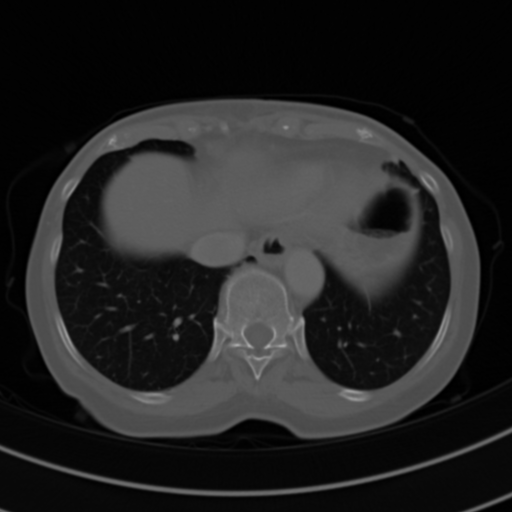
\includegraphics[width=9cm]{1-11.png}};
	\node at (44, 1.5)  {\Huge \(R(f, \phi)\)};
\end{tikzpicture}
\end{document}
